\documentclass[12pt]{article}\usepackage[]{graphicx}\usepackage[]{color}
%% maxwidth is the original width if it is less than linewidth
%% otherwise use linewidth (to make sure the graphics do not exceed the margin)
\makeatletter
\def\maxwidth{ %
  \ifdim\Gin@nat@width>\linewidth
    \linewidth
  \else
    \Gin@nat@width
  \fi
}
\makeatother

\definecolor{fgcolor}{rgb}{0.345, 0.345, 0.345}
\newcommand{\hlnum}[1]{\textcolor[rgb]{0.686,0.059,0.569}{#1}}%
\newcommand{\hlstr}[1]{\textcolor[rgb]{0.192,0.494,0.8}{#1}}%
\newcommand{\hlcom}[1]{\textcolor[rgb]{0.678,0.584,0.686}{\textit{#1}}}%
\newcommand{\hlopt}[1]{\textcolor[rgb]{0,0,0}{#1}}%
\newcommand{\hlstd}[1]{\textcolor[rgb]{0.345,0.345,0.345}{#1}}%
\newcommand{\hlkwa}[1]{\textcolor[rgb]{0.161,0.373,0.58}{\textbf{#1}}}%
\newcommand{\hlkwb}[1]{\textcolor[rgb]{0.69,0.353,0.396}{#1}}%
\newcommand{\hlkwc}[1]{\textcolor[rgb]{0.333,0.667,0.333}{#1}}%
\newcommand{\hlkwd}[1]{\textcolor[rgb]{0.737,0.353,0.396}{\textbf{#1}}}%
\let\hlipl\hlkwb

\usepackage{framed}
\makeatletter
\newenvironment{kframe}{%
 \def\at@end@of@kframe{}%
 \ifinner\ifhmode%
  \def\at@end@of@kframe{\end{minipage}}%
  \begin{minipage}{\columnwidth}%
 \fi\fi%
 \def\FrameCommand##1{\hskip\@totalleftmargin \hskip-\fboxsep
 \colorbox{shadecolor}{##1}\hskip-\fboxsep
     % There is no \\@totalrightmargin, so:
     \hskip-\linewidth \hskip-\@totalleftmargin \hskip\columnwidth}%
 \MakeFramed {\advance\hsize-\width
   \@totalleftmargin\z@ \linewidth\hsize
   \@setminipage}}%
 {\par\unskip\endMakeFramed%
 \at@end@of@kframe}
\makeatother

\definecolor{shadecolor}{rgb}{.97, .97, .97}
\definecolor{messagecolor}{rgb}{0, 0, 0}
\definecolor{warningcolor}{rgb}{1, 0, 1}
\definecolor{errorcolor}{rgb}{1, 0, 0}
\newenvironment{knitrout}{}{} % an empty environment to be redefined in TeX

\usepackage{alltt}
 
\usepackage[margin=1in]{geometry}
\usepackage{amsmath,amsthm,amssymb, mathtools}
\usepackage[T1]{fontenc}
\usepackage{lmodern}
\usepackage{fixltx2e}
\usepackage[shortlabels]{enumitem}
\usepackage{mathrsfs}
 
\newcommand{\N}{\mathbb{N}}
\newcommand{\R}{\mathbb{R}}
\newcommand{\Z}{\mathbb{Z}}
\newcommand{\Q}{\mathbb{Q}}
 
\newenvironment{theorem}[2][Theorem]{\begin{trivlist}
\item[\hskip \labelsep {\bfseries #1}\hskip \labelsep {\bfseries #2.}]}{\end{trivlist}}
\newenvironment{lemma}[2][Lemma]{\begin{trivlist}
\item[\hskip \labelsep {\bfseries #1}\hskip \labelsep {\bfseries #2.}]}{\end{trivlist}}
\newenvironment{exercise}[2][Exercise]{\begin{trivlist}
\item[\hskip \labelsep {\bfseries #1}\hskip \labelsep {\bfseries #2.}]}{\end{trivlist}}
\newenvironment{problem}[2][Problem]{\begin{trivlist}
\item[\hskip \labelsep {\bfseries #1}\hskip \labelsep {\bfseries #2.}]}{\end{trivlist}}
\newenvironment{question}[2][Question]{\begin{trivlist}
\item[\hskip \labelsep {\bfseries #1}\hskip \labelsep {\bfseries #2.}]}{\end{trivlist}}
\newenvironment{corollary}[2][Corollary]{\begin{trivlist}
\item[\hskip \labelsep {\bfseries #1}\hskip \labelsep {\bfseries #2.}]}{\end{trivlist}}
\newcommand{\textfrac}[2]{\dfrac{\text{#1}}{\text{#2}}}

\DeclareMathOperator{\proj}{proj}
\newcommand{\vct}{\mathbf}
\newcommand{\vctproj}[2][]{\proj_{\vct{#1}}\vct{#2}}
\IfFileExists{upquote.sty}{\usepackage{upquote}}{}
\begin{document}

\title{Advanced Mathematical Statistics: Assignment 3}

\author{Chris Hayduk}
\date{October 10, 2019}

\maketitle



\section{Problems to be Completed}

\begin{problem}{4.23}
\end{problem}

\begin{enumerate}[a)]

\item Let $\vct{X}' = \begin{bmatrix} -0.6 & 3.1 & 25.3 & -16.8 & -7.1 & -6.2 & 16.1 & 25.2 & 22.6 & 26.0 \end{bmatrix}$.\\

In order to construct a Q-Q plot for the data, we need to compute the quantiles for the data as well as the quantiles for the theoretical normal distribution. Then we can plot the ordered data against the theoretical quantile as an ordered pair. After doing so, we can assess the whether the distribution is normal by checking the linearity of the plot. In order to do this, I will use the R programming language.

\begin{knitrout}
\definecolor{shadecolor}{rgb}{0.969, 0.969, 0.969}\color{fgcolor}\begin{kframe}
\begin{alltt}
\hlcom{#Create data vector}
\hlstd{x} \hlkwb{<-} \hlkwd{c}\hlstd{(}\hlopt{-}\hlnum{0.6}\hlstd{,} \hlnum{3.1}\hlstd{,} \hlnum{25.3}\hlstd{,} \hlopt{-}\hlnum{16.8}\hlstd{,} \hlopt{-}\hlnum{7.1}\hlstd{,} \hlopt{-}\hlnum{6.2}\hlstd{,} \hlnum{16.1}\hlstd{,} \hlnum{25.2}\hlstd{,} \hlnum{22.6}\hlstd{,} \hlnum{26.0}\hlstd{)}

\hlcom{#Sort data}
\hlstd{x} \hlkwb{<-} \hlkwd{sort}\hlstd{(x)}

\hlcom{#Let n = # of observations}
\hlstd{n} \hlkwb{<-} \hlkwd{length}\hlstd{(x)}

\hlcom{#Output sample size}
\hlstd{n}
\end{alltt}
\begin{verbatim}
## [1] 10
\end{verbatim}
\begin{alltt}
\hlcom{#Calculate the quantiles for the actual data}
\hlstd{prob_levels} \hlkwb{<-} \hlstd{((}\hlnum{1}\hlopt{:}\hlstd{n)}\hlopt{-}\hlnum{0.5}\hlstd{)}\hlopt{/}\hlstd{n}

\hlcom{#Calculate the theoretical normal quantiles}
\hlstd{standard_normal_quantiles} \hlkwb{<-} \hlkwd{qnorm}\hlstd{(prob_levels)}

\hlcom{#Round the theoretical quantiles to 2 decimal places}
\hlstd{standard_normal_quantiles} \hlkwb{<-} \hlkwd{round}\hlstd{(standard_normal_quantiles,}
                                   \hlkwc{digits} \hlstd{=} \hlnum{2}\hlstd{)}

\hlcom{#Create matrix of values}
\hlstd{qq_matrix} \hlkwb{<-} \hlkwd{as.data.frame}\hlstd{(}\hlkwd{cbind}\hlstd{(x, prob_levels,}
                                 \hlstd{standard_normal_quantiles))}

\hlcom{#Print matrix}
\hlstd{qq_matrix}
\end{alltt}
\begin{verbatim}
##        x prob_levels standard_normal_quantiles
## 1  -16.8        0.05                     -1.64
## 2   -7.1        0.15                     -1.04
## 3   -6.2        0.25                     -0.67
## 4   -0.6        0.35                     -0.39
## 5    3.1        0.45                     -0.13
## 6   16.1        0.55                      0.13
## 7   22.6        0.65                      0.39
## 8   25.2        0.75                      0.67
## 9   25.3        0.85                      1.04
## 10  26.0        0.95                      1.64
\end{verbatim}
\end{kframe}
\end{knitrout}

Now that we have the data required to construct the Q-Q plot, we will use R to plot the ordered data against the theoretical quantiles. We will also include a line of best fit in order to see if the sample and theoretical quantiles are linearily related.

\begin{knitrout}
\definecolor{shadecolor}{rgb}{0.969, 0.969, 0.969}\color{fgcolor}\begin{kframe}
\begin{alltt}
\hlkwd{ggplot}\hlstd{(qq_matrix,} \hlkwd{aes}\hlstd{(standard_normal_quantiles, x))} \hlopt{+}
  \hlkwd{geom_point}\hlstd{(}\hlkwc{size}\hlstd{=}\hlnum{3}\hlstd{)} \hlopt{+}
  \hlkwd{geom_smooth}\hlstd{(}\hlkwc{method}\hlstd{=}\hlstr{'lm'}\hlstd{,} \hlkwc{se}\hlstd{=F)} \hlopt{+}
  \hlkwd{xlab}\hlstd{(}\hlstr{"Theoretical Quantiles"}\hlstd{)} \hlopt{+}
  \hlkwd{ylab}\hlstd{(}\hlstr{"Ordered Data"}\hlstd{)} \hlopt{+}
  \hlkwd{ggtitle}\hlstd{(}\hlstr{"Q-Q Plot"}\hlstd{)} \hlopt{+}
  \hlstd{theme.info}
\end{alltt}
\end{kframe}
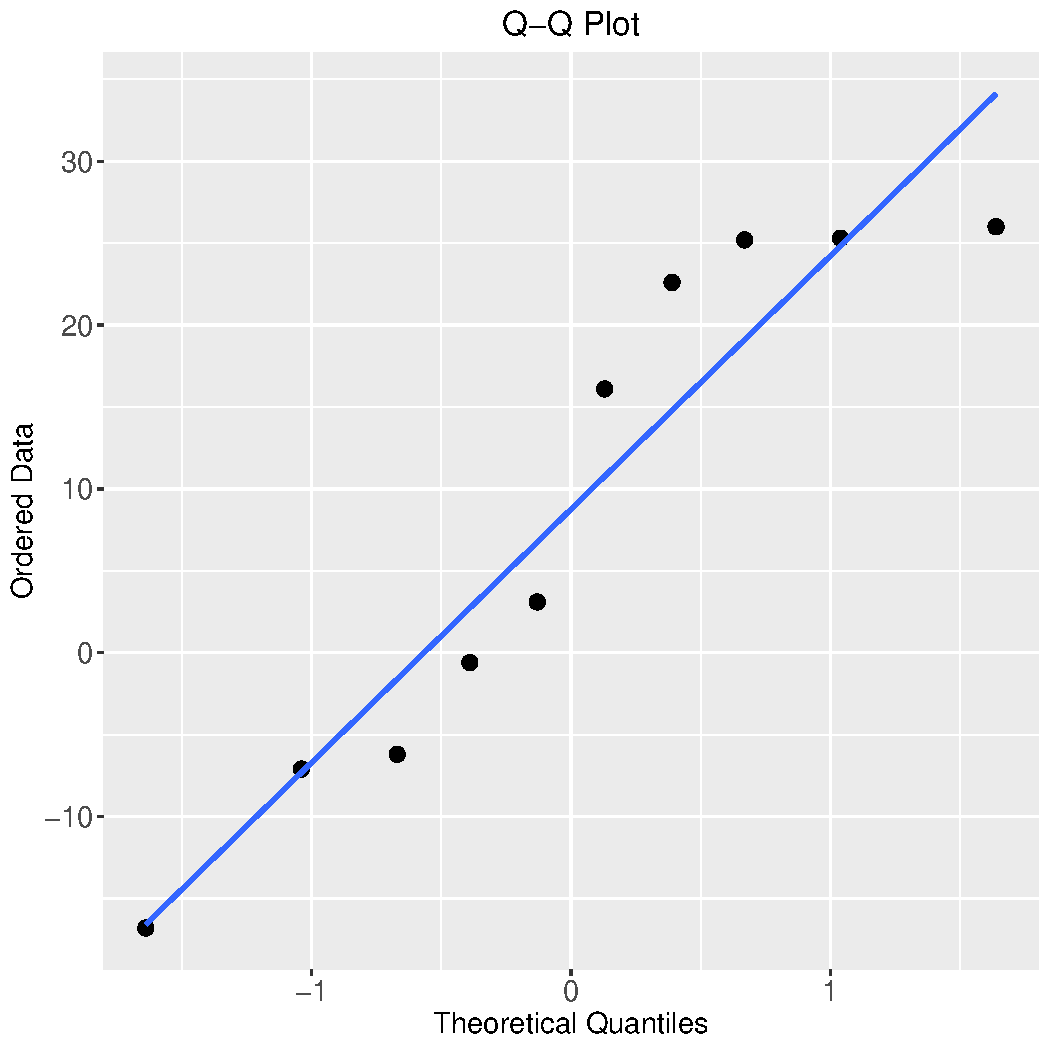
\includegraphics[width=\maxwidth]{figure/unnamed-chunk-3-1} 

\end{knitrout}

There do not appear to be any large deviations from the line of best fit, so it is reasonable to assume that the data is in fact normally distributed.

\item We will use R to compute the correlation coefficient between the standard normal quantiles and the sample quantiles.

\begin{knitrout}
\definecolor{shadecolor}{rgb}{0.969, 0.969, 0.969}\color{fgcolor}\begin{kframe}
\begin{alltt}
\hlcom{#Calculate mean of data}
\hlstd{x_bar} \hlkwb{<-} \hlkwd{mean}\hlstd{(qq_matrix}\hlopt{$}\hlstd{x)}

\hlcom{#Calculate three components of correlation equation separately }
\hlcom{#(as in Example 4.11 in textbook)}
\hlstd{part1} \hlkwb{<-} \hlkwd{sum}\hlstd{((qq_matrix}\hlopt{$}\hlstd{x} \hlopt{-} \hlstd{x_bar)}\hlopt{*}\hlstd{qq_matrix}\hlopt{$}\hlstd{standard_normal_quantiles)}
\hlstd{part2} \hlkwb{<-} \hlkwd{sum}\hlstd{((qq_matrix}\hlopt{$}\hlstd{x} \hlopt{-} \hlstd{x_bar)}\hlopt{^}\hlnum{2}\hlstd{)}
\hlstd{part3} \hlkwb{<-} \hlkwd{sum}\hlstd{((qq_matrix}\hlopt{$}\hlstd{standard_normal_quantiles)}\hlopt{^}\hlnum{2}\hlstd{)}

\hlcom{#Compute correlation}
\hlstd{r_Q} \hlkwb{<-} \hlstd{part1}\hlopt{/}\hlstd{(}\hlkwd{sqrt}\hlstd{(part2)}\hlopt{*}\hlkwd{sqrt}\hlstd{(part3))}

\hlcom{#Output correlation}
\hlstd{r_Q}
\end{alltt}
\begin{verbatim}
## [1] 0.9476294
\end{verbatim}
\begin{alltt}
\hlcom{#Check against R's built in correlation function}
\hlkwd{cor}\hlstd{(qq_matrix}\hlopt{$}\hlstd{x, qq_matrix}\hlopt{$}\hlstd{standard_normal_quantiles)}
\end{alltt}
\begin{verbatim}
## [1] 0.9476294
\end{verbatim}
\end{kframe}
\end{knitrout}

From Table 4.2, for a sample size of 10 and $\alpha = 0.1$, the correlation needs to be at least 0.9351 in order for us to not reject the hypothesis of normality. As can be seen from the computation above, the correlation coefficient between the data and the standard normal quantiles is greater than the threshold value. Thus, we cannot reject the hypothesis of normality.

\end{enumerate}

%%%%%%%%%%%%%%%%%%%%%%%%%%%%%%%%%%%%%%%%%%%%%%%%%%%%%%%%%%%%%%%%%%%%%%%%%%%%%%%%%%%%%%%%%%%%%%%%%%%%%%%%%%%%%%%%%%%%%%%%%%%%%%%%%%%%%

\begin{problem}{4.24}
\end{problem}

\begin{enumerate}[a)]

\item We will construct the Q-Q plots as in the above exercise. First, we will begin with the sales data.

\begin{knitrout}
\definecolor{shadecolor}{rgb}{0.969, 0.969, 0.969}\color{fgcolor}\begin{kframe}
\begin{alltt}
\hlcom{#Create data vector}
\hlstd{sales} \hlkwb{<-} \hlkwd{c}\hlstd{(}\hlnum{108.28}\hlstd{,} \hlnum{152.36}\hlstd{,} \hlnum{95.04}\hlstd{,} \hlnum{65.45}\hlstd{,} \hlnum{62.97}\hlstd{,}
           \hlnum{263.99}\hlstd{,} \hlnum{265.19}\hlstd{,} \hlnum{285.06}\hlstd{,} \hlnum{92.01}\hlstd{,} \hlnum{165.68}\hlstd{)}
\hlstd{x} \hlkwb{<-} \hlstd{sales}

\hlcom{#Sort data}
\hlstd{x} \hlkwb{<-} \hlkwd{sort}\hlstd{(x)}

\hlcom{#Let n = # of observations}
\hlstd{n} \hlkwb{<-} \hlkwd{length}\hlstd{(x)}

\hlcom{#Output sample size}
\hlstd{n}
\end{alltt}
\begin{verbatim}
## [1] 10
\end{verbatim}
\begin{alltt}
\hlcom{#Calculate the quantiles for the actual data}
\hlstd{prob_levels} \hlkwb{<-} \hlstd{((}\hlnum{1}\hlopt{:}\hlstd{n)}\hlopt{-}\hlnum{0.5}\hlstd{)}\hlopt{/}\hlstd{n}

\hlcom{#Calculate the theoretical normal quantiles}
\hlstd{standard_normal_quantiles} \hlkwb{<-} \hlkwd{qnorm}\hlstd{(prob_levels)}

\hlcom{#Round the theoretical quantiles to 2 decimal places}
\hlstd{standard_normal_quantiles} \hlkwb{<-} \hlkwd{round}\hlstd{(standard_normal_quantiles,}
                                   \hlkwc{digits} \hlstd{=} \hlnum{2}\hlstd{)}

\hlcom{#Create matrix of values}
\hlstd{qq_matrix1} \hlkwb{<-} \hlkwd{as.data.frame}\hlstd{(}\hlkwd{cbind}\hlstd{(x, prob_levels,}
                                 \hlstd{standard_normal_quantiles))}

\hlcom{#Print matrix}
\hlstd{qq_matrix1}
\end{alltt}
\begin{verbatim}
##         x prob_levels standard_normal_quantiles
## 1   62.97        0.05                     -1.64
## 2   65.45        0.15                     -1.04
## 3   92.01        0.25                     -0.67
## 4   95.04        0.35                     -0.39
## 5  108.28        0.45                     -0.13
## 6  152.36        0.55                      0.13
## 7  165.68        0.65                      0.39
## 8  263.99        0.75                      0.67
## 9  265.19        0.85                      1.04
## 10 285.06        0.95                      1.64
\end{verbatim}
\begin{alltt}
\hlcom{#Output plot}
\hlkwd{ggplot}\hlstd{(qq_matrix1,} \hlkwd{aes}\hlstd{(standard_normal_quantiles, x))} \hlopt{+}
  \hlkwd{geom_point}\hlstd{(}\hlkwc{size}\hlstd{=}\hlnum{3}\hlstd{)} \hlopt{+}
  \hlkwd{geom_smooth}\hlstd{(}\hlkwc{method}\hlstd{=}\hlstr{'lm'}\hlstd{,} \hlkwc{se}\hlstd{=F)} \hlopt{+}
  \hlkwd{xlab}\hlstd{(}\hlstr{"Theoretical Quantiles"}\hlstd{)} \hlopt{+}
  \hlkwd{ylab}\hlstd{(}\hlstr{"Ordered Data"}\hlstd{)} \hlopt{+}
  \hlkwd{ggtitle}\hlstd{(}\hlstr{"Q-Q Plot for Sales Data"}\hlstd{)} \hlopt{+}
  \hlstd{theme.info}
\end{alltt}
\end{kframe}
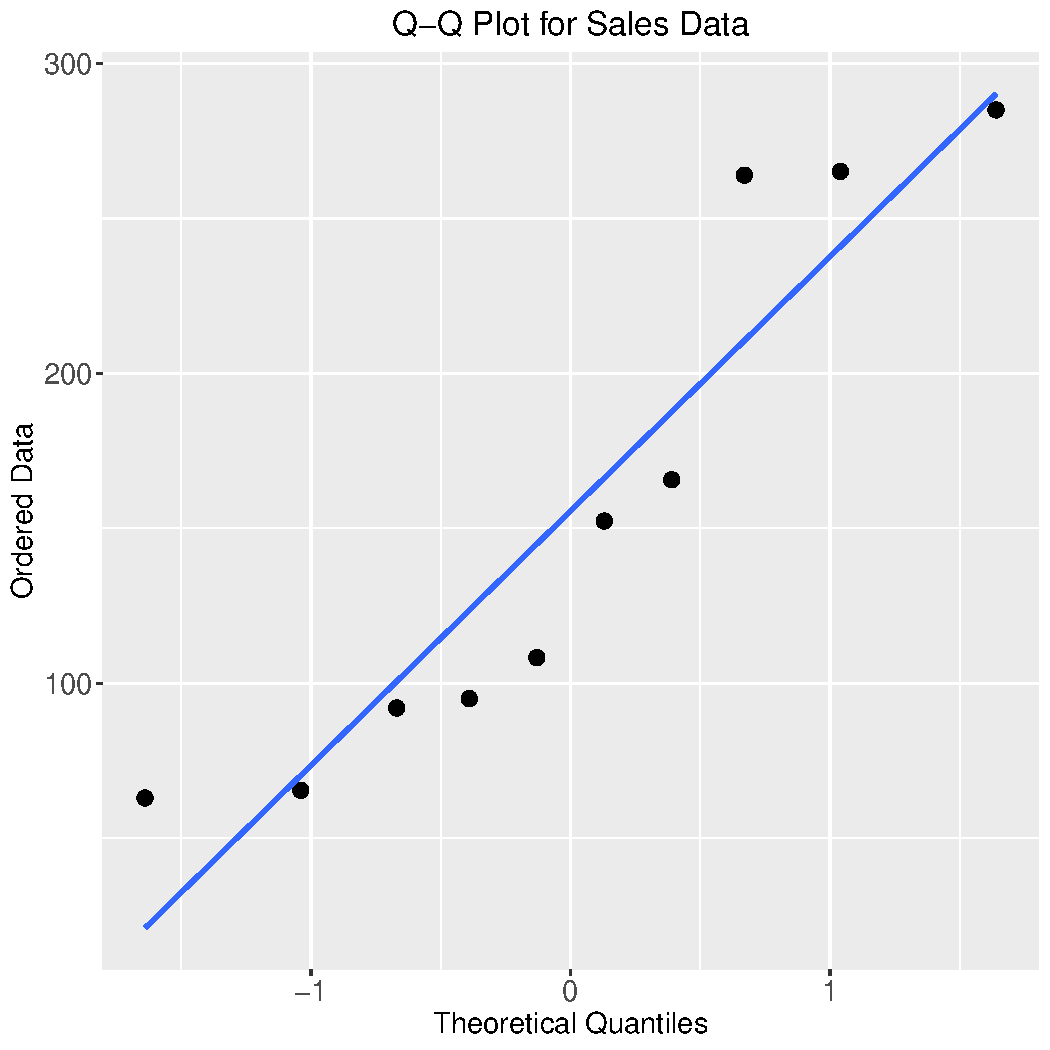
\includegraphics[width=\maxwidth]{figure/unnamed-chunk-5-1} 

\end{knitrout}

Most of the points appear close to the line of best fit. However, there are a couple points that may be considered significant outliers. As a result, it is difficult to say whether the data is normally distributed.

Now, we will perform the same analysis for the profits data.

\begin{knitrout}
\definecolor{shadecolor}{rgb}{0.969, 0.969, 0.969}\color{fgcolor}\begin{kframe}
\begin{alltt}
\hlcom{#Create data vector}
\hlstd{profits} \hlkwb{<-} \hlkwd{c}\hlstd{(}\hlnum{17.05}\hlstd{,} \hlnum{16.59}\hlstd{,} \hlnum{10.91}\hlstd{,} \hlnum{14.14}\hlstd{,} \hlnum{9.52}\hlstd{,}
             \hlnum{25.33}\hlstd{,} \hlnum{18.54}\hlstd{,} \hlnum{15.73}\hlstd{,} \hlnum{8.10}\hlstd{,} \hlnum{11.13}\hlstd{)}
\hlstd{x} \hlkwb{<-} \hlstd{profits}

\hlcom{#Sort data}
\hlstd{x} \hlkwb{<-} \hlkwd{sort}\hlstd{(x)}

\hlcom{#Let n = # of observations}
\hlstd{n} \hlkwb{<-} \hlkwd{length}\hlstd{(x)}

\hlcom{#Output sample size}
\hlstd{n}
\end{alltt}
\begin{verbatim}
## [1] 10
\end{verbatim}
\begin{alltt}
\hlcom{#Calculate the quantiles for the actual data}
\hlstd{prob_levels} \hlkwb{<-} \hlstd{((}\hlnum{1}\hlopt{:}\hlstd{n)}\hlopt{-}\hlnum{0.5}\hlstd{)}\hlopt{/}\hlstd{n}

\hlcom{#Calculate the theoretical normal quantiles}
\hlstd{standard_normal_quantiles} \hlkwb{<-} \hlkwd{qnorm}\hlstd{(prob_levels)}

\hlcom{#Round the theoretical quantiles to 2 decimal places}
\hlstd{standard_normal_quantiles} \hlkwb{<-} \hlkwd{round}\hlstd{(standard_normal_quantiles,}
                                   \hlkwc{digits} \hlstd{=} \hlnum{2}\hlstd{)}

\hlcom{#Create matrix of values}
\hlstd{qq_matrix2} \hlkwb{<-} \hlkwd{as.data.frame}\hlstd{(}\hlkwd{cbind}\hlstd{(x, prob_levels,}
                                 \hlstd{standard_normal_quantiles))}

\hlcom{#Print matrix}
\hlstd{qq_matrix2}
\end{alltt}
\begin{verbatim}
##        x prob_levels standard_normal_quantiles
## 1   8.10        0.05                     -1.64
## 2   9.52        0.15                     -1.04
## 3  10.91        0.25                     -0.67
## 4  11.13        0.35                     -0.39
## 5  14.14        0.45                     -0.13
## 6  15.73        0.55                      0.13
## 7  16.59        0.65                      0.39
## 8  17.05        0.75                      0.67
## 9  18.54        0.85                      1.04
## 10 25.33        0.95                      1.64
\end{verbatim}
\begin{alltt}
\hlcom{#Output plot}
\hlkwd{ggplot}\hlstd{(qq_matrix2,} \hlkwd{aes}\hlstd{(standard_normal_quantiles, x))} \hlopt{+}
  \hlkwd{geom_point}\hlstd{(}\hlkwc{size}\hlstd{=}\hlnum{3}\hlstd{)} \hlopt{+}
  \hlkwd{geom_smooth}\hlstd{(}\hlkwc{method}\hlstd{=}\hlstr{'lm'}\hlstd{,} \hlkwc{se}\hlstd{=F)} \hlopt{+}
  \hlkwd{xlab}\hlstd{(}\hlstr{"Theoretical Quantiles"}\hlstd{)} \hlopt{+}
  \hlkwd{ylab}\hlstd{(}\hlstr{"Ordered Data"}\hlstd{)} \hlopt{+}
  \hlkwd{ggtitle}\hlstd{(}\hlstr{"Q-Q Plot for Profit Data"}\hlstd{)} \hlopt{+}
  \hlstd{theme.info}
\end{alltt}
\end{kframe}
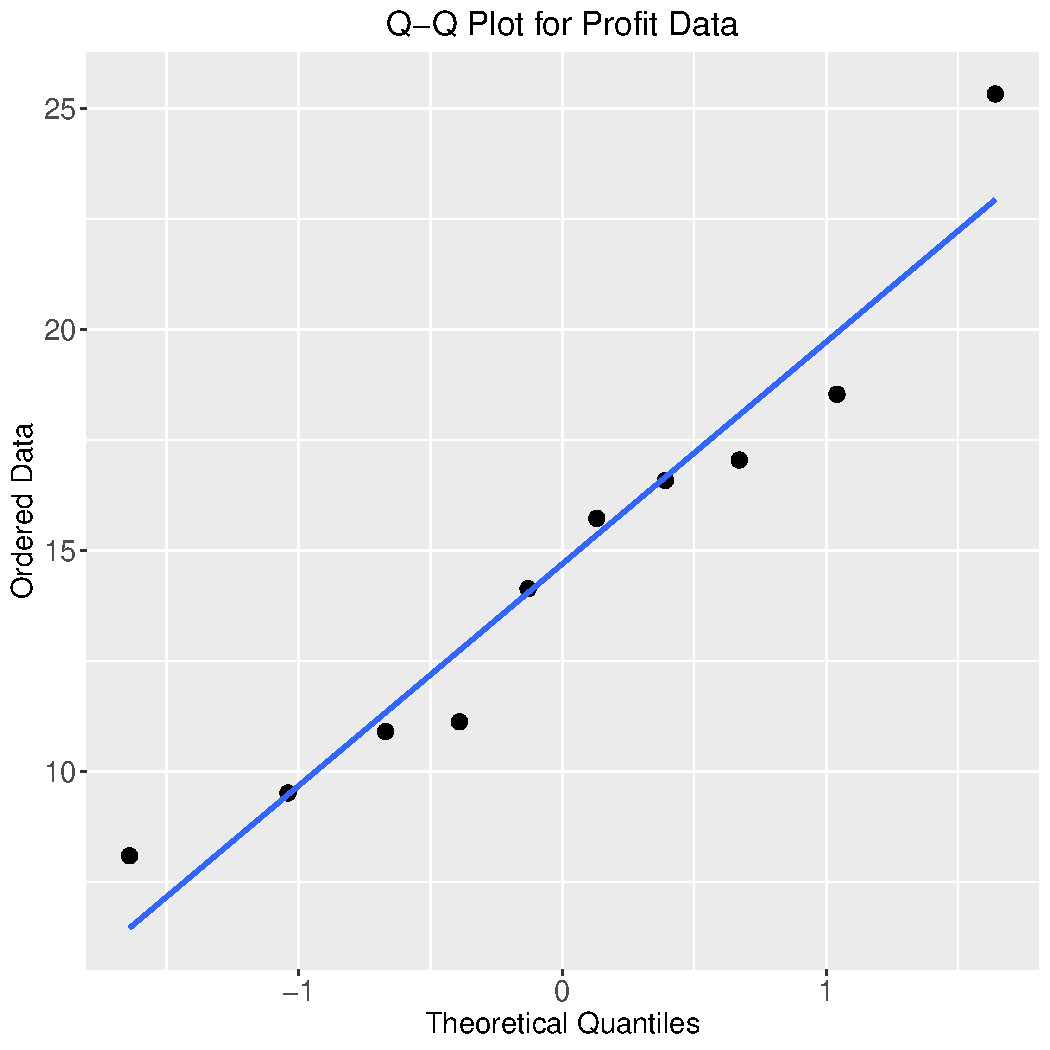
\includegraphics[width=\maxwidth]{figure/unnamed-chunk-6-1} 

\end{knitrout}

The points in this plot appear to closely follow the line of best fit. Thus, the data is likely normally distributed.

\item We will now perform correlation analysis for each of the two data vectors. We will again begin with the sales data.

\begin{knitrout}
\definecolor{shadecolor}{rgb}{0.969, 0.969, 0.969}\color{fgcolor}\begin{kframe}
\begin{alltt}
\hlcom{#Calculate mean of data}
\hlstd{x_bar} \hlkwb{<-} \hlkwd{mean}\hlstd{(qq_matrix1}\hlopt{$}\hlstd{x)}

\hlcom{#Calculate three components of correlation equation separately }
\hlcom{#(as in Example 4.11 in textbook)}
\hlstd{part1} \hlkwb{<-} \hlkwd{sum}\hlstd{((qq_matrix1}\hlopt{$}\hlstd{x} \hlopt{-} \hlstd{x_bar)}\hlopt{*}\hlstd{qq_matrix1}\hlopt{$}\hlstd{standard_normal_quantiles)}
\hlstd{part2} \hlkwb{<-} \hlkwd{sum}\hlstd{((qq_matrix1}\hlopt{$}\hlstd{x} \hlopt{-} \hlstd{x_bar)}\hlopt{^}\hlnum{2}\hlstd{)}
\hlstd{part3} \hlkwb{<-} \hlkwd{sum}\hlstd{((qq_matrix1}\hlopt{$}\hlstd{standard_normal_quantiles)}\hlopt{^}\hlnum{2}\hlstd{)}

\hlcom{#Compute correlation}
\hlstd{r_Q} \hlkwb{<-} \hlstd{part1}\hlopt{/}\hlstd{(}\hlkwd{sqrt}\hlstd{(part2)}\hlopt{*}\hlkwd{sqrt}\hlstd{(part3))}

\hlcom{#Output correlation}
\hlstd{r_Q}
\end{alltt}
\begin{verbatim}
## [1] 0.9374333
\end{verbatim}
\begin{alltt}
\hlcom{#Check against R's built in correlation function}
\hlkwd{cor}\hlstd{(qq_matrix1}\hlopt{$}\hlstd{x, qq_matrix1}\hlopt{$}\hlstd{standard_normal_quantiles)}
\end{alltt}
\begin{verbatim}
## [1] 0.9374333
\end{verbatim}
\end{kframe}
\end{knitrout}

From Table 4.2, for a sample size of 10 and $\alpha = 0.1$, the correlation needs to be at least 0.9351 in order for us to not reject the hypothesis of normality. As can be seen from the computation above, the correlation coefficient between the sales data and the standard normal quantiles is greater than the threshold value. Thus, we cannot reject the hypothesis of normality.\\

We will now perform the same analysis for the profit data.

\begin{knitrout}
\definecolor{shadecolor}{rgb}{0.969, 0.969, 0.969}\color{fgcolor}\begin{kframe}
\begin{alltt}
\hlcom{#Calculate mean of data}
\hlstd{x_bar} \hlkwb{<-} \hlkwd{mean}\hlstd{(qq_matrix2}\hlopt{$}\hlstd{x)}

\hlcom{#Calculate three components of correlation equation separately }
\hlcom{#(as in Example 4.11 in textbook)}
\hlstd{part1} \hlkwb{<-} \hlkwd{sum}\hlstd{((qq_matrix2}\hlopt{$}\hlstd{x} \hlopt{-} \hlstd{x_bar)}\hlopt{*}\hlstd{qq_matrix2}\hlopt{$}\hlstd{standard_normal_quantiles)}
\hlstd{part2} \hlkwb{<-} \hlkwd{sum}\hlstd{((qq_matrix2}\hlopt{$}\hlstd{x} \hlopt{-} \hlstd{x_bar)}\hlopt{^}\hlnum{2}\hlstd{)}
\hlstd{part3} \hlkwb{<-} \hlkwd{sum}\hlstd{((qq_matrix2}\hlopt{$}\hlstd{standard_normal_quantiles)}\hlopt{^}\hlnum{2}\hlstd{)}

\hlcom{#Compute correlation}
\hlstd{r_Q} \hlkwb{<-} \hlstd{part1}\hlopt{/}\hlstd{(}\hlkwd{sqrt}\hlstd{(part2)}\hlopt{*}\hlkwd{sqrt}\hlstd{(part3))}

\hlcom{#Output correlation}
\hlstd{r_Q}
\end{alltt}
\begin{verbatim}
## [1] 0.969226
\end{verbatim}
\begin{alltt}
\hlcom{#Check against R's built in correlation function}
\hlkwd{cor}\hlstd{(qq_matrix2}\hlopt{$}\hlstd{x, qq_matrix2}\hlopt{$}\hlstd{standard_normal_quantiles)}
\end{alltt}
\begin{verbatim}
## [1] 0.969226
\end{verbatim}
\end{kframe}
\end{knitrout}

From Table 4.2, for a sample size of 10 and $\alpha = 0.1$, the correlation needs to be at least 0.9351 in order for us to not reject the hypothesis of normality. As can be seen from the computation above, the correlation coefficient between the profit data and the standard normal quantiles is greater than the threshold value. Thus, we cannot reject the hypothesis of normality.\\

The above correlation values agree with our visual assessment of the Q-Q plots. Both the plots do not indicate that the data is not normally distributed, with the profit data Q-Q plot appearing to deviate from the line of best fit less than the sales data Q-Q plot. The correlation values provide a similar analysis, with both data sets meeting the correlation threshold, while the profit data exhibited a stronger correlation with the theoretical quantiles.

\end{enumerate}

%%%%%%%%%%%%%%%%%%%%%%%%%%%%%%%%%%%%%%%%%%%%%%%%%%%%%%%%%%%%%%%%%%%%%%%%%%%%%%%%%%%%%%%%%%%%%%%%%%%%%%%%%%%%%%%%%%%%%%%%%%%%%%%%%%%%%

\begin{problem}{4.25}
\end{problem}

We will again use the R programming language, this time to compute a Chi-Square plot for the data from Exercise 1.4.

\begin{knitrout}
\definecolor{shadecolor}{rgb}{0.969, 0.969, 0.969}\color{fgcolor}\begin{kframe}
\begin{alltt}
\hlcom{#Create data matrix}
\hlstd{data} \hlkwb{<-} \hlkwd{matrix}\hlstd{(}\hlkwd{c}\hlstd{(}\hlnum{108.28}\hlstd{,} \hlnum{17.05}\hlstd{,} \hlnum{1484.10}\hlstd{,} \hlnum{152.36}\hlstd{,} \hlnum{16.59}\hlstd{,}
                 \hlnum{750.33}\hlstd{,} \hlnum{95.04}\hlstd{,} \hlnum{10.91}\hlstd{,} \hlnum{766.42}\hlstd{,} \hlnum{65.45}\hlstd{,}
                 \hlnum{14.14}\hlstd{,} \hlnum{1110.46}\hlstd{,} \hlnum{62.97}\hlstd{,} \hlnum{9.52}\hlstd{,} \hlnum{1031.29}\hlstd{,}
                 \hlnum{263.99}\hlstd{,} \hlnum{25.33}\hlstd{,} \hlnum{195.26}\hlstd{,} \hlnum{265.19}\hlstd{,} \hlnum{18.54}\hlstd{,}
                 \hlnum{193.83}\hlstd{,} \hlnum{285.06}\hlstd{,} \hlnum{15.73}\hlstd{,} \hlnum{191.11}\hlstd{,} \hlnum{92.01}\hlstd{,}
                 \hlnum{8.10}\hlstd{,} \hlnum{1175.16}\hlstd{,} \hlnum{165.68}\hlstd{,} \hlnum{11.13}\hlstd{,} \hlnum{211.15}\hlstd{),}
               \hlkwc{nrow} \hlstd{=} \hlnum{10}\hlstd{,} \hlkwc{ncol} \hlstd{=} \hlnum{3}\hlstd{,} \hlkwc{byrow}\hlstd{=} \hlnum{TRUE}\hlstd{)}

\hlcom{#Get mean of each variable}
\hlstd{means} \hlkwb{<-} \hlkwd{apply}\hlstd{(data,} \hlnum{2}\hlstd{, mean)}

\hlkwd{print}\hlstd{(means)}
\end{alltt}
\begin{verbatim}
## [1] 155.603  14.704 710.911
\end{verbatim}
\begin{alltt}
\hlcom{#Create matrix of means for subtraction purposes}
\hlstd{means_matrix} \hlkwb{<-} \hlkwd{matrix}\hlstd{(}\hlkwc{data} \hlstd{=} \hlkwd{rep}\hlstd{(means,} \hlkwc{times} \hlstd{=} \hlnum{10}\hlstd{),}
                       \hlkwc{nrow} \hlstd{=} \hlnum{10}\hlstd{,} \hlkwc{ncol} \hlstd{=} \hlnum{3}\hlstd{,} \hlkwc{byrow} \hlstd{=} \hlnum{TRUE}\hlstd{)}

\hlcom{#Subtract mean from data}
\hlstd{data_minus_mean} \hlkwb{<-} \hlstd{data} \hlopt{-} \hlstd{means_matrix}

\hlkwd{print}\hlstd{(data_minus_mean)}
\end{alltt}
\begin{verbatim}
##          [,1]   [,2]     [,3]
##  [1,] -47.323  2.346  773.189
##  [2,]  -3.243  1.886   39.419
##  [3,] -60.563 -3.794   55.509
##  [4,] -90.153 -0.564  399.549
##  [5,] -92.633 -5.184  320.379
##  [6,] 108.387 10.626 -515.651
##  [7,] 109.587  3.836 -517.081
##  [8,] 129.457  1.026 -519.801
##  [9,] -63.593 -6.604  464.249
## [10,]  10.077 -3.574 -499.761
\end{verbatim}
\begin{alltt}
\hlcom{#Get covariance matrix}
\hlstd{S} \hlkwb{<-} \hlkwd{cov}\hlstd{(data)}

\hlcom{#Get inverse of covariance matrix}
\hlstd{S_inv} \hlkwb{<-} \hlkwd{as.matrix}\hlstd{(}\hlkwd{inv}\hlstd{(S))}

\hlcom{#Create vector to store distance values}
\hlstd{d} \hlkwb{<-} \hlkwd{rep}\hlstd{(}\hlnum{0}\hlstd{,} \hlkwc{times} \hlstd{=} \hlnum{10}\hlstd{)}

\hlcom{#Compute distance values}
\hlkwa{for}\hlstd{(i} \hlkwa{in} \hlnum{1}\hlopt{:}\hlkwd{nrow}\hlstd{(data_minus_mean))\{}
  \hlstd{d[i]} \hlkwb{<-} \hlstd{(}\hlkwd{t}\hlstd{(data_minus_mean[i,])} \hlopt \hlstd{S_inv} \hlopt \hlstd{(data_minus_mean[i,]))}
\hlstd{\}}

\hlcom{#Sort the distances}
\hlstd{d} \hlkwb{<-} \hlkwd{sort}\hlstd{(d)}

\hlstd{d}
\end{alltt}
\begin{verbatim}
##  [1] 0.3142218 1.2894389 1.4070422 1.6411732 2.0191102 3.0405613 3.1884264
##  [8] 4.3513949 4.8347957 4.9084233
\end{verbatim}
\begin{alltt}
\hlcom{#Chi-square quantiles from textbook exercise}
\hlstd{chisq_quantiles} \hlkwb{<-} \hlkwd{c}\hlstd{(}\hlnum{0.3518}\hlstd{,} \hlnum{0.7978}\hlstd{,} \hlnum{1.2125}\hlstd{,} \hlnum{1.6416}\hlstd{,}
                     \hlnum{2.1095}\hlstd{,} \hlnum{2.6430}\hlstd{,} \hlnum{3.2831}\hlstd{,} \hlnum{4.1083}\hlstd{,}
                     \hlnum{5.3170}\hlstd{,} \hlnum{7.8147}\hlstd{)}

\hlcom{#Create data frame for plot}
\hlstd{chisq_plot} \hlkwb{<-} \hlkwd{as.data.frame}\hlstd{(}\hlkwd{cbind}\hlstd{(d, chisq_quantiles))}

\hlcom{#Output plot}
\hlkwd{ggplot}\hlstd{(chisq_plot,} \hlkwd{aes}\hlstd{(chisq_quantiles, d))} \hlopt{+}
  \hlkwd{geom_point}\hlstd{(}\hlkwc{size}\hlstd{=}\hlnum{3}\hlstd{)} \hlopt{+}
  \hlkwd{geom_smooth}\hlstd{(}\hlkwc{method}\hlstd{=}\hlstr{'lm'}\hlstd{,} \hlkwc{se}\hlstd{=F)} \hlopt{+}
  \hlkwd{xlab}\hlstd{(}\hlstr{"Theoretical Quantiles"}\hlstd{)} \hlopt{+}
  \hlkwd{ylab}\hlstd{(}\hlstr{"Ordered Distances"}\hlstd{)} \hlopt{+}
  \hlkwd{ggtitle}\hlstd{(}\hlstr{"Chi-Square Plot"}\hlstd{)} \hlopt{+}
  \hlstd{theme.info}
\end{alltt}
\end{kframe}
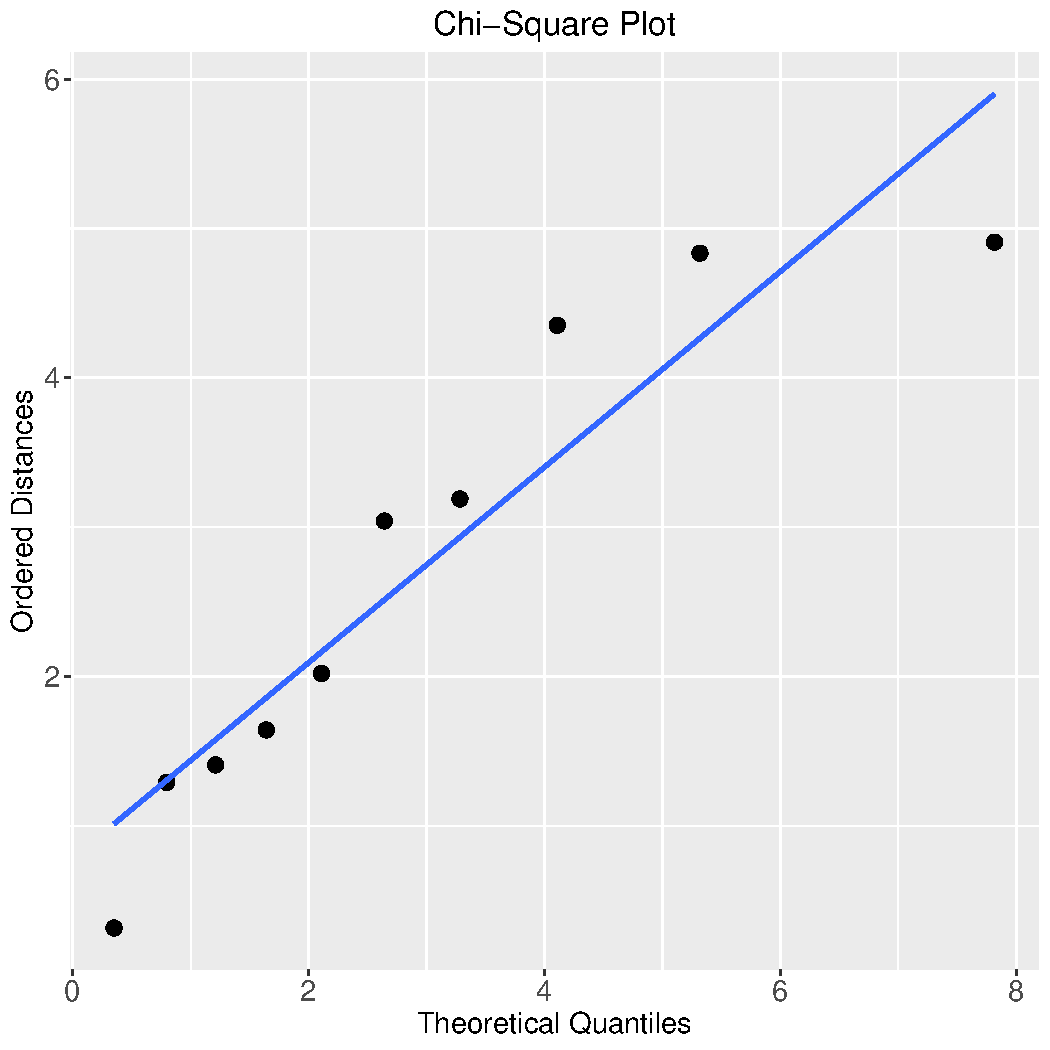
\includegraphics[width=\maxwidth]{figure/unnamed-chunk-9-1} 

\end{knitrout}

Given the sample size, it is difficult to reject trivariate normality based upon the evidence in this graph.

%%%%%%%%%%%%%%%%%%%%%%%%%%%%%%%%%%%%%%%%%%%%%%%%%%%%%%%%%%%%%%%%%%%%%%%%%%%%%%%%%%%%%%%%%%%%%%%%%%%%%%%%%%%%%%%%%%%%%%%%%%%%%%%%%%%%%
\newpage
\begin{problem}{4.30}
\end{problem}

For this problem, we will be implementing the Box-Cox solution in order to find an appropriate power for $\lambda$. I will implement a function here so that this can be performed repeatedly.

\begin{knitrout}
\definecolor{shadecolor}{rgb}{0.969, 0.969, 0.969}\color{fgcolor}\begin{kframe}
\begin{alltt}
\hlstd{box_cox} \hlkwb{<-} \hlkwa{function}\hlstd{(}\hlkwc{data}\hlstd{,} \hlkwc{lambda}\hlstd{,} \hlkwc{n}\hlstd{)\{}
  \hlcom{#Create vector to store values for l of lambda}
  \hlstd{l_of_lambda} \hlkwb{<-} \hlkwd{rep}\hlstd{(}\hlopt{-}\hlnum{100}\hlstd{,} \hlkwc{times} \hlstd{=} \hlkwd{length}\hlstd{(lambda))}

  \hlcom{#For loop to calculate l of lambda}
  \hlkwa{for}\hlstd{(i} \hlkwa{in} \hlnum{1}\hlopt{:}\hlkwd{length}\hlstd{(lambda))\{}
    \hlcom{#Check if lambda is equal to 0}
    \hlkwa{if}\hlstd{(lambda[i]} \hlopt{!=} \hlnum{0}\hlstd{)\{}
      \hlstd{y} \hlkwb{<-} \hlstd{(data}\hlopt{^}\hlstd{(lambda[i])} \hlopt{-} \hlnum{1}\hlstd{)}\hlopt{/}\hlstd{lambda[i]}
    \hlstd{\}} \hlkwa{else}\hlstd{\{}
      \hlstd{y} \hlkwb{<-} \hlkwd{log}\hlstd{(data)}
    \hlstd{\}}

    \hlcom{#Calculate mean of transformed x_1 values}
    \hlstd{y_bar} \hlkwb{<-} \hlkwd{mean}\hlstd{(y)}

    \hlcom{#Calculate value for l of lambda function and store it in the vector}
    \hlstd{l_of_lambda[i]} \hlkwb{<-} \hlstd{(}\hlopt{-}\hlstd{n}\hlopt{/}\hlnum{2}\hlstd{)}\hlopt{*}\hlkwd{log}\hlstd{((}\hlnum{1}\hlopt{/}\hlstd{n)} \hlopt{*} \hlkwd{sum}\hlstd{((y} \hlopt{-} \hlstd{y_bar)}\hlopt{^}\hlnum{2}\hlstd{))} \hlopt{+}
      \hlstd{(lambda[i]} \hlopt{-} \hlnum{1}\hlstd{)} \hlopt{*} \hlkwd{sum}\hlstd{(}\hlkwd{log}\hlstd{(data))}
  \hlstd{\}}

  \hlcom{#Find the lambda value that corresponds to the max value of l of lambda}
  \hlstd{lambda_final} \hlkwb{<-} \hlstd{lambda[}\hlkwd{which.max}\hlstd{(l_of_lambda)]}

  \hlkwd{return}\hlstd{(lambda_final)}
\hlstd{\}}
\end{alltt}
\end{kframe}
\end{knitrout}

Furthermore, we will be using the same $\lambda$ vectors and $n$ values for all parts of this problem, so I will define those here:

\begin{knitrout}
\definecolor{shadecolor}{rgb}{0.969, 0.969, 0.969}\color{fgcolor}\begin{kframe}
\begin{alltt}
\hlcom{#Create vector of possible lambda values}
\hlstd{lambda} \hlkwb{<-} \hlkwd{seq}\hlstd{(}\hlkwc{from} \hlstd{=} \hlopt{-}\hlnum{5.00}\hlstd{,} \hlkwc{to} \hlstd{=} \hlnum{5.00}\hlstd{,} \hlkwc{by} \hlstd{=} \hlnum{0.01}\hlstd{)}

\hlcom{#Let n = length of x_1 vector}
\hlstd{n} \hlkwb{<-} \hlnum{10}
\end{alltt}
\end{kframe}
\end{knitrout}

Now, we can move on to computing these transformations.

\begin{enumerate}[a)]

\item We will begin by finding the power transformation $\hat{\lambda}_1$ that makes the $x_1$ values approximately normal.

\begin{knitrout}
\definecolor{shadecolor}{rgb}{0.969, 0.969, 0.969}\color{fgcolor}\begin{kframe}
\begin{alltt}
\hlcom{#Create vector of x_1 values}
\hlstd{x_1} \hlkwb{<-} \hlkwd{c}\hlstd{(}\hlnum{1}\hlstd{,} \hlnum{2}\hlstd{,} \hlnum{3}\hlstd{,} \hlnum{3}\hlstd{,} \hlnum{4}\hlstd{,} \hlnum{5}\hlstd{,} \hlnum{6}\hlstd{,} \hlnum{8}\hlstd{,} \hlnum{9}\hlstd{,} \hlnum{11}\hlstd{)}

\hlcom{#Find lambda value}
\hlstd{lambda_final} \hlkwb{<-} \hlkwd{box_cox}\hlstd{(x_1, lambda, n)}

\hlstd{lambda_final}
\end{alltt}
\begin{verbatim}
## [1] 0.37
\end{verbatim}
\begin{alltt}
\hlcom{#Transform x_1 using this lambda value}
\hlstd{transformed_x_1} \hlkwb{<-} \hlstd{(x_1}\hlopt{^}\hlstd{lambda_final} \hlopt{-} \hlnum{1}\hlstd{)}\hlopt{/}\hlstd{lambda_final}

\hlstd{transformed_x_1} \hlkwb{<-} \hlkwd{sort}\hlstd{(transformed_x_1)}

\hlcom{#Calculate the quantiles for the actual data}
\hlstd{prob_levels} \hlkwb{<-} \hlstd{((}\hlnum{1}\hlopt{:}\hlstd{n)}\hlopt{-}\hlnum{0.5}\hlstd{)}\hlopt{/}\hlstd{n}

\hlcom{#Calculate the theoretical normal quantiles}
\hlstd{standard_normal_quantiles} \hlkwb{<-} \hlkwd{qnorm}\hlstd{(prob_levels)}

\hlcom{#Round the theoretical quantiles to 2 decimal places}
\hlstd{standard_normal_quantiles} \hlkwb{<-} \hlkwd{round}\hlstd{(standard_normal_quantiles,}
                                   \hlkwc{digits} \hlstd{=} \hlnum{2}\hlstd{)}

\hlcom{#Create matrix of values}
\hlstd{qq_matrix} \hlkwb{<-} \hlkwd{as.data.frame}\hlstd{(}\hlkwd{cbind}\hlstd{(transformed_x_1, prob_levels,}
                                 \hlstd{standard_normal_quantiles))}

\hlcom{#Print matrix}
\hlstd{qq_matrix}
\end{alltt}
\begin{verbatim}
##    transformed_x_1 prob_levels standard_normal_quantiles
## 1        0.0000000        0.05                     -1.64
## 2        0.7901428        0.15                     -1.04
## 3        1.3554944        0.25                     -0.67
## 4        1.3554944        0.35                     -0.39
## 5        1.8112861        0.45                     -0.13
## 6        2.1997925        0.55                      0.13
## 7        2.5419199        0.65                      0.39
## 8        3.1309634        0.75                      0.67
## 9        3.3908140        0.85                      1.04
## 10       3.8604660        0.95                      1.64
\end{verbatim}
\begin{alltt}
\hlcom{#Output plot}
\hlkwd{ggplot}\hlstd{(qq_matrix,} \hlkwd{aes}\hlstd{(standard_normal_quantiles, transformed_x_1))} \hlopt{+}
  \hlkwd{geom_point}\hlstd{(}\hlkwc{size}\hlstd{=}\hlnum{3}\hlstd{)} \hlopt{+}
  \hlkwd{geom_smooth}\hlstd{(}\hlkwc{method}\hlstd{=}\hlstr{'lm'}\hlstd{,} \hlkwc{se}\hlstd{=F)} \hlopt{+}
  \hlkwd{xlab}\hlstd{(}\hlstr{"Theoretical Quantiles"}\hlstd{)} \hlopt{+}
  \hlkwd{ylab}\hlstd{(}\hlstr{"Ordered Data"}\hlstd{)} \hlopt{+}
  \hlkwd{ggtitle}\hlstd{(}\hlkwd{TeX}\hlstd{(}\hlstr{'Q-Q Plot for $x_1$'}\hlstd{))} \hlopt{+}
  \hlstd{theme.info}
\end{alltt}
\end{kframe}
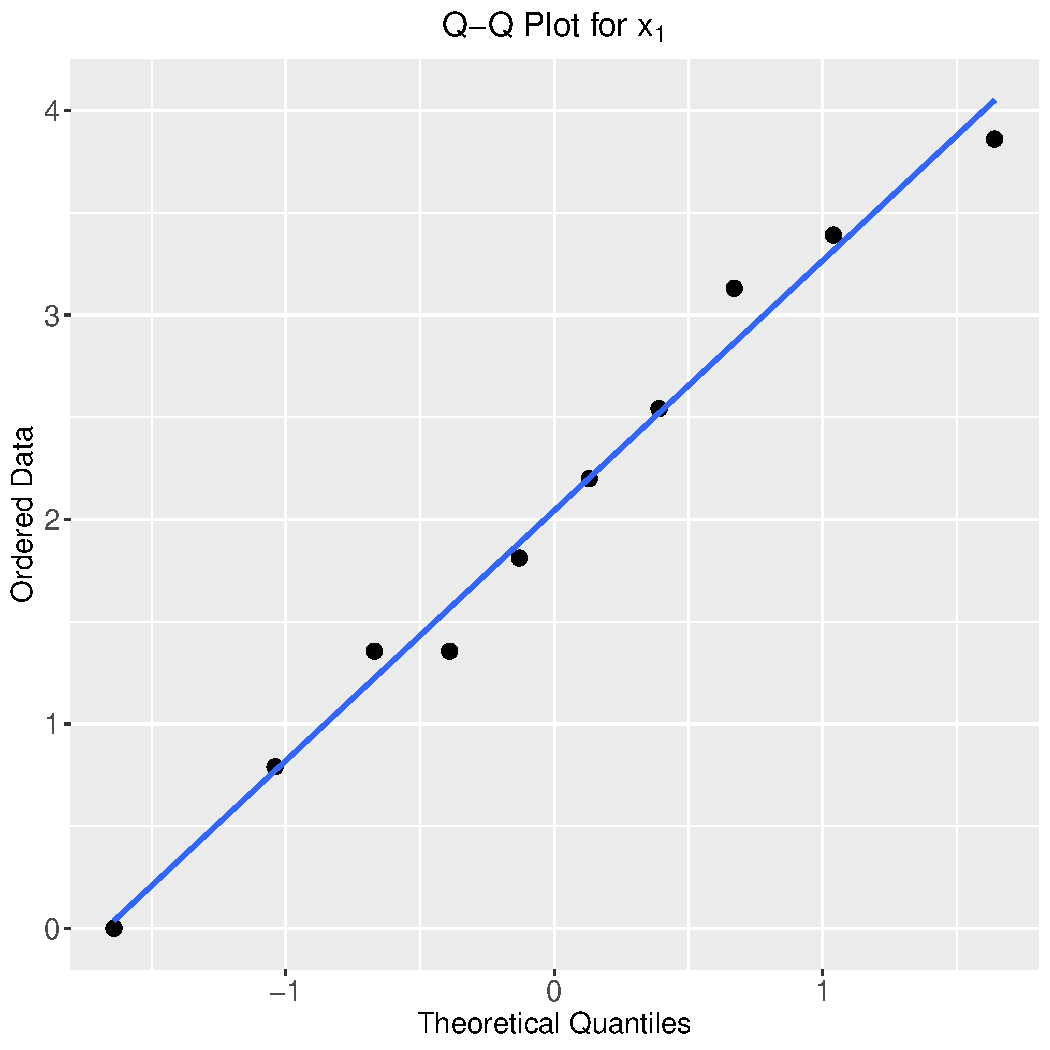
\includegraphics[width=\maxwidth]{figure/unnamed-chunk-12-1} 

\end{knitrout}

From the above, we have $\hat{\lambda}_1$ = 0.37. As we can see from the Q-Q plot, this transformation has caused the data to be distributed approximately normally. 

\item Now we will find the power transformation $\hat{\lambda}_2$ that makes the $x_2$ values approximately normal.

\begin{knitrout}
\definecolor{shadecolor}{rgb}{0.969, 0.969, 0.969}\color{fgcolor}\begin{kframe}
\begin{alltt}
\hlcom{#Create vector of x_2 values}
\hlstd{x_2} \hlkwb{<-} \hlkwd{c}\hlstd{(}\hlnum{18.95}\hlstd{,} \hlnum{19.00}\hlstd{,} \hlnum{17.95}\hlstd{,} \hlnum{15.54}\hlstd{,}
         \hlnum{14.00}\hlstd{,} \hlnum{12.95}\hlstd{,} \hlnum{8.94}\hlstd{,} \hlnum{7.49}\hlstd{,} \hlnum{6.00}\hlstd{,} \hlnum{3.99}\hlstd{)}

\hlcom{#Find lambda value}
\hlstd{lambda_final} \hlkwb{<-} \hlkwd{box_cox}\hlstd{(x_2, lambda, n)}

\hlstd{lambda_final}
\end{alltt}
\begin{verbatim}
## [1] 0.94
\end{verbatim}
\begin{alltt}
\hlcom{#Transform x_2 using this lambda value}
\hlstd{transformed_x_2} \hlkwb{<-} \hlstd{(x_2}\hlopt{^}\hlstd{lambda_final} \hlopt{-} \hlnum{1}\hlstd{)}\hlopt{/}\hlstd{lambda_final}

\hlstd{transformed_x_2} \hlkwb{<-} \hlkwd{sort}\hlstd{(transformed_x_2)}

\hlcom{#Calculate the quantiles for the actual data}
\hlstd{prob_levels} \hlkwb{<-} \hlstd{((}\hlnum{1}\hlopt{:}\hlstd{n)}\hlopt{-}\hlnum{0.5}\hlstd{)}\hlopt{/}\hlstd{n}

\hlcom{#Calculate the theoretical normal quantiles}
\hlstd{standard_normal_quantiles} \hlkwb{<-} \hlkwd{qnorm}\hlstd{(prob_levels)}

\hlcom{#Round the theoretical quantiles to 2 decimal places}
\hlstd{standard_normal_quantiles} \hlkwb{<-} \hlkwd{round}\hlstd{(standard_normal_quantiles,}
                                   \hlkwc{digits} \hlstd{=} \hlnum{2}\hlstd{)}

\hlcom{#Create matrix of values}
\hlstd{qq_matrix} \hlkwb{<-} \hlkwd{as.data.frame}\hlstd{(}\hlkwd{cbind}\hlstd{(transformed_x_2, prob_levels,}
                                 \hlstd{standard_normal_quantiles))}

\hlcom{#Print matrix}
\hlstd{qq_matrix}
\end{alltt}
\begin{verbatim}
##    transformed_x_2 prob_levels standard_normal_quantiles
## 1         2.842660        0.05                     -1.64
## 2         4.668542        0.15                     -1.04
## 3         5.997477        0.25                     -0.67
## 4         7.275467        0.35                     -0.39
## 5        10.750409        0.45                     -0.13
## 6        11.648715        0.55                      0.13
## 7        12.959014        0.65                      0.39
## 8        14.994217        0.75                      0.67
## 9        15.833762        0.85                      1.04
## 10       15.875668        0.95                      1.64
\end{verbatim}
\begin{alltt}
\hlcom{#Output plot}
\hlkwd{ggplot}\hlstd{(qq_matrix,} \hlkwd{aes}\hlstd{(standard_normal_quantiles, transformed_x_2))} \hlopt{+}
  \hlkwd{geom_point}\hlstd{(}\hlkwc{size}\hlstd{=}\hlnum{3}\hlstd{)} \hlopt{+}
  \hlkwd{geom_smooth}\hlstd{(}\hlkwc{method}\hlstd{=}\hlstr{'lm'}\hlstd{,} \hlkwc{se}\hlstd{=F)} \hlopt{+}
  \hlkwd{xlab}\hlstd{(}\hlstr{"Theoretical Quantiles"}\hlstd{)} \hlopt{+}
  \hlkwd{ylab}\hlstd{(}\hlstr{"Ordered Data"}\hlstd{)} \hlopt{+}
  \hlkwd{ggtitle}\hlstd{(}\hlkwd{TeX}\hlstd{(}\hlstr{'Q-Q Plot for $x_2$'}\hlstd{))} \hlopt{+}
  \hlstd{theme.info}
\end{alltt}
\end{kframe}
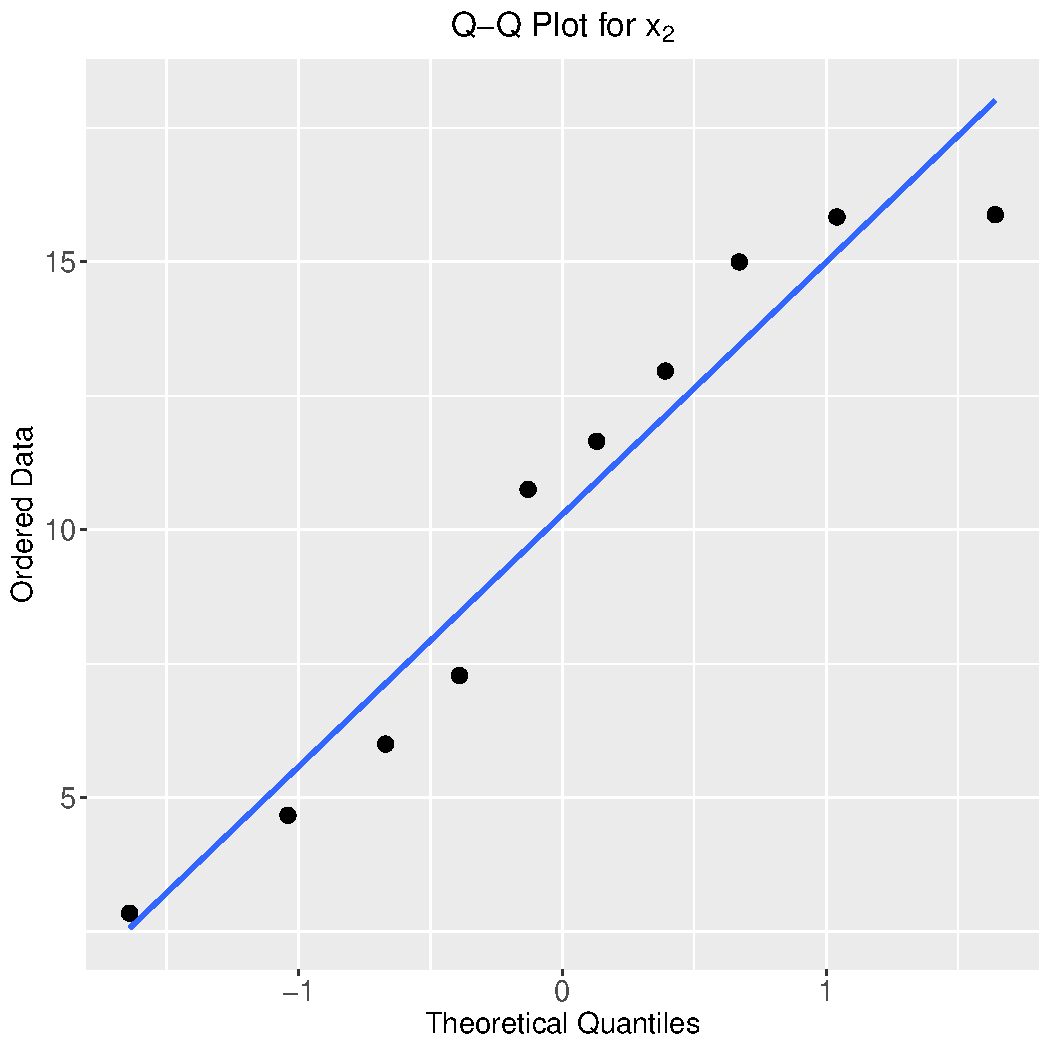
\includegraphics[width=\maxwidth]{figure/unnamed-chunk-13-1} 

\end{knitrout}

From the above, we have $\hat{\lambda}_2$ = 0.94. As we can see from the Q-Q plot, this transformation has caused the data to be distributed approximately normally. 

\item We will compute $\vct{\hat{\lambda}'} = \begin{bmatrix} \hat{\lambda_1} & \hat{\lambda_2} \end{bmatrix}$ over a large grid of points in order to determine the appropriate transformation to make the $[x_1, x_2]$ values jointly normal.

\begin{knitrout}
\definecolor{shadecolor}{rgb}{0.969, 0.969, 0.969}\color{fgcolor}\begin{kframe}
\begin{alltt}
\hlcom{#Length of sequence for lambda values}
\hlstd{ng} \hlkwb{<-} \hlnum{400}

\hlcom{#Size of lambda matrix}
\hlstd{n2} \hlkwb{<-} \hlstd{ng}\hlopt{^}\hlnum{2}

\hlcom{#Create lambda vectors}
\hlstd{lambda_1} \hlkwb{<-} \hlkwd{seq}\hlstd{(}\hlnum{0.0001}\hlstd{,} \hlnum{2.00}\hlstd{,} \hlkwc{len} \hlstd{= ng)}
\hlstd{lambda_2} \hlkwb{<-} \hlkwd{seq}\hlstd{(}\hlnum{0.0001}\hlstd{,} \hlnum{2.00}\hlstd{,} \hlkwc{len} \hlstd{= ng)}

\hlcom{#Repeat lambda values}
\hlstd{lambda_1} \hlkwb{<-} \hlkwd{outer}\hlstd{(lambda_1,} \hlkwd{rep}\hlstd{(}\hlnum{1}\hlstd{, ng))}
\hlstd{lambda_2} \hlkwb{<-} \hlkwd{outer}\hlstd{(}\hlkwd{rep}\hlstd{(}\hlnum{1}\hlstd{,ng), lambda_2)}

\hlcom{#Form grid of lambda values}
\hlstd{lambda_matrix} \hlkwb{<-} \hlkwd{cbind}\hlstd{(lambda_1[}\hlnum{1}\hlopt{:}\hlstd{n2], lambda_2[}\hlnum{1}\hlopt{:}\hlstd{n2])}

\hlcom{#Create vector to store function values}
\hlstd{l_of_lambda_vec} \hlkwb{<-} \hlkwd{rep}\hlstd{(}\hlnum{0}\hlstd{,} \hlkwc{times} \hlstd{=} \hlkwd{nrow}\hlstd{(lambda_matrix))}

\hlcom{#Create matrix of x values}
\hlstd{x} \hlkwb{<-} \hlkwd{cbind}\hlstd{(x_1, x_2)}

\hlcom{#For loop for function}
\hlkwa{for}\hlstd{(i} \hlkwa{in} \hlnum{1}\hlopt{:}\hlkwd{nrow}\hlstd{(lambda_matrix))\{}
  \hlcom{#Get lambda values from grid}
  \hlstd{lambda_vals} \hlkwb{<-} \hlstd{lambda_matrix[i, ]}

  \hlcom{#Compute transformed x matrix}
  \hlstd{transformed_x} \hlkwb{<-} \hlkwd{cbind}\hlstd{((x[,}\hlnum{1}\hlstd{]}\hlopt{^}\hlstd{(lambda_vals[}\hlnum{1}\hlstd{])} \hlopt{-} \hlnum{1}\hlstd{)}\hlopt{/}\hlstd{lambda_vals[}\hlnum{1}\hlstd{],}
                         \hlstd{(x[,}\hlnum{2}\hlstd{]}\hlopt{^}\hlstd{(lambda_vals[}\hlnum{2}\hlstd{])} \hlopt{-} \hlnum{1}\hlstd{)}\hlopt{/}\hlstd{lambda_vals[}\hlnum{2}\hlstd{])}

  \hlcom{#Compute covariance of transformed x matrix}
  \hlstd{S} \hlkwb{<-} \hlkwd{cov}\hlstd{(transformed_x)}

  \hlcom{#Compute determinant of covariance}
  \hlstd{det_S} \hlkwb{<-} \hlkwd{det}\hlstd{(S)}

  \hlcom{#Calculate function value and store it in vector}
  \hlstd{l_of_lambda_vec[i]} \hlkwb{<-} \hlstd{(}\hlopt{-}\hlstd{n}\hlopt{/}\hlnum{2}\hlstd{)} \hlopt{*} \hlkwd{log}\hlstd{(det_S)} \hlopt{+}
    \hlstd{(lambda_vals[}\hlnum{1}\hlstd{]} \hlopt{-} \hlnum{1}\hlstd{)} \hlopt{*} \hlkwd{sum}\hlstd{(}\hlkwd{log}\hlstd{(x[,}\hlnum{1}\hlstd{]))} \hlopt{+}
    \hlstd{(lambda_vals[}\hlnum{2}\hlstd{]} \hlopt{-} \hlnum{1}\hlstd{)} \hlopt{*} \hlkwd{sum}\hlstd{(}\hlkwd{log}\hlstd{(x[,}\hlnum{2}\hlstd{]))}
\hlstd{\}}

\hlcom{#Find the lambda vector that gives the max value of l of lambda}
\hlstd{lambda_vec_final} \hlkwb{<-} \hlstd{lambda_matrix[}\hlkwd{which.max}\hlstd{(l_of_lambda_vec),]}

\hlkwd{print}\hlstd{(lambda_vec_final)}
\end{alltt}
\begin{verbatim}
## [1] 1.27321930 0.03017368
\end{verbatim}
\end{kframe}
\end{knitrout}

From the above, we have that $\vct{\hat{\lambda}'} = \begin{bmatrix} 1.2732 & 0.0302 \end{bmatrix}$. Surprisingly, these values differ significantly from the values obtained in the calculations for the marginal distributions of $x_1$ and $x_2$.

\end{enumerate}

%%%%%%%%%%%%%%%%%%%%%%%%%%%%%%%%%%%%%%%%%%%%%%%%%%%%%%%%%%%%%%%%%%%%%%%%%%%%%%%%%%%%%%%%%%%%%%%%%%%%%%%%%%%%%%%%%%%%%%%%%%%%%%%%%%%%%
%%%%%%%%%%%%%%%%%%%%%%%%%%%%%%%%%%%%%%%%%%%%%%%%%%%%%%%%%%%%%%%%%%%%%%%%%%%%%%%%%%%%%%%%%%%%%%%%%%%%%%%%%%%%%%%%%%%%%%%%%%%%%%%%%%%%%
%%%%%%%%%%%%%%%%%%%%%%%%%%%%%%%%%%%%%%%%%%%%%%%%%%%%%%%%%%%%%%%%%%%%%%%%%%%%%%%%%%%%%%%%%%%%%%%%%%%%%%%%%%%%%%%%%%%%%%%%%%%%%%%%%%%%%

\section{Problems to be Described}

\begin{problem}{4.28}
\end{problem}

For this question, we would construct a Q-Q plot and compute the resulting correlation coefficient, as we did in problems 4.23 and 4.24.

%%%%%%%%%%%%%%%%%%%%%%%%%%%%%%%%%%%%%%%%%%%%%%%%%%%%%%%%%%%%%%%%%%%%%%%%%%%%%%%%%%%%%%%%%%%%%%%%%%%%%%%%%%%%%%%%%%%%%%%%%%%%%%%%%%%%%

\begin{problem}{4.32}
\end{problem}

We could first construct Q-Q plots for each of the variables $X_1, ... X_6$. For any variable $X_k$ that appears to not be normally distributed, we could find the value $\lambda_k$ that maximizes the Box-Cox equation. We could then apply this $\lambda_k$ transformation to the variable, construct another Q-Q plot, and assess its normality once again.

%%%%%%%%%%%%%%%%%%%%%%%%%%%%%%%%%%%%%%%%%%%%%%%%%%%%%%%%%%%%%%%%%%%%%%%%%%%%%%%%%%%%%%%%%%%%%%%%%%%%%%%%%%%%%%%%%%%%%%%%%%%%%%%%%%%%%

\begin{problem}{4.34}
\end{problem}

First, construct Q-Q plots for each variable. If either appears to not be normally distributed, use the Box-Cox formula to find and apply a transformation to it, then reassess its normality through a Q-Q plot.\\

Next, construct a Chi-square plot to assess the bivariate normality of the data. If it does not appear to be normally distributed, use the joint Box-Cox formula to find a transformation for the joint distribution. Apply this transformation and construct another Chi-square plot in order to assess normality.

%%%%%%%%%%%%%%%%%%%%%%%%%%%%%%%%%%%%%%%%%%%%%%%%%%%%%%%%%%%%%%%%%%%%%%%%%%%%%%%%%%%%%%%%%%%%%%%%%%%%%%%%%%%%%%%%%%%%%%%%%%%%%%%%%%%%%

\begin{problem}{4.35}
\end{problem}

Once again, construct Q-Q plots for each variable. If any appear to not be normally distributed, use the Box-Cox formula to find and apply a transformation to it, then reassess its normality through a Q-Q plot.\\

Next, construct a Chi-square plot to assess the multivariate normality of the data. If it does not appear to be normally distributed, use the joint Box-Cox formula to find a transformation for the joint distribution. Apply this transformation and construct another Chi-square plot in order to assess normality.

%%%%%%%%%%%%%%%%%%%%%%%%%%%%%%%%%%%%%%%%%%%%%%%%%%%%%%%%%%%%%%%%%%%%%%%%%%%%%%%%%%%%%%%%%%%%%%%%%%%%%%%%%%%%%%%%%%%%%%%%%%%%%%%%%%%%%

\begin{problem}{4.39(a)(b)}
\end{problem}

\begin{enumerate}[a)]

\item Construct Q-Q plots for each variable. If any appear to not be normally distributed, use the Box-Cox formula to find and apply a transformation to it, then reassess its normality through a Q-Q plot.

\item Construct a Chi-square plot to assess the multivariate normality of the data. If it does not appear to be normally distributed, use the joint Box-Cox formula to find a transformation for the joint distribution. Apply this transformation and construct another Chi-square plot in order to assess normality.

\end{enumerate}

%%%%%%%%%%%%%%%%%%%%%%%%%%%%%%%%%%%%%%%%%%%%%%%%%%%%%%%%%%%%%%%%%%%%%%%%%%%%%%%%%%%%%%%%%%%%%%%%%%%%%%%%%%%%%%%%%%%%%%%%%%%%%%%%%%%%%

\begin{problem}{4.40}
\end{problem}

\begin{enumerate}[a)]

\item Construct scatter plots for each pair of variables and calculate the generalized squared distance for each observation in order to identify outliers.

\item Use the univariate Box-Cox formula to identify a $\hat{\lambda}_1$ value. Then construct a Q-Q plot.

\item Use the univariate Box-Cox formula to identify a $\hat{\lambda}_2$ value. Then construct a Q-Q plot.

\item Use the joint Box-Cox formula to identify a $\vct{\hat{\lambda}}$ value.

\end{enumerate}

%%%%%%%%%%%%%%%%%%%%%%%%%%%%%%%%%%%%%%%%%%%%%%%%%%%%%%%%%%%%%%%%%%%%%%%%%%%%%%%%%%%%%%%%%%%%%%%%%%%%%%%%%%%%%%%%%%%%%%%%%%%%%%%%%%%%%

\begin{problem}{4.41}
\end{problem}

\begin{enumerate}[a)]

\item Construct scatter plots for each pair of variables and calculate the generalized squared distance for each observation in order to identify outliers.

\item Use the univariate Box-Cox formula to identify a $\hat{\lambda}_1$ value. Then construct a Q-Q plot.

\item Use the univariate Box-Cox formula to identify a $\hat{\lambda}_2$ value. Then construct a Q-Q plot.

\item Use the joint Box-Cox formula to identify a $\vct{\hat{\lambda}}$ value.

\end{enumerate}
\end{document}
